%%%%%%%%%%%%%%%%%%%%%%%%%%%%%
%Since : 2018/11/13
%Update: <2019/03/07>
% -*- coding: utf-8 -*-
%%%%%%%%%%%%%%%%%%%%%%%%%%%%%
\documentclass[12pt, a4j]{jreport}
\usepackage[dvipdfmx]{graphicx}
%\usepackage{graphicx}
\usepackage{amsmath}
\usepackage{amssymb}
\usepackage{cite}

\renewcommand{\prechaptername}{第}
\renewcommand{\postchaptername}{回}
\renewcommand{\thesection}{\arabic{section}}

\title{Excelによる統計処理実習}
\author{公立小松大学臨床工学科 \\ 藤田 一寿}
\date{}

\begin{document}

\maketitle

\chapter{Excelによる統計処理1}

\section{目的}

Excelの操作を通し,データ処理の基礎とグラフの作成の仕方を学ぶ.

\section{理論}

\subsection{統計とは}

統計や確率は様々な場面で用いられています.
それはなぜでしょうか.
一つの目的は,全体の特徴もしくは規則性を捉えるために用いられます.
皆さんは,大学受験で出てきた様々な統計量に触れてきたのではないでしょうか.
大学の偏差値もその一つで,合格者の集団特性を表したものです.
今後,卒業研究はもちろん就職してからも大量のデータを扱うことになると思います.
そこで,そのデータの特徴を捉えるために用いるのが統計です.
この演習を通じ,その基礎を身につけてください.

\subsection{データ}

$N$個のデータがあるとするとその集合$X$は次のように表されます.
\begin{equation}
    \label{eq:2}
    X = \{x_1, x_2, ..., x_N\}
\end{equation}

\subsection{代表値}

例えば,表\ref{tab:sample}に示すデータがあったとします.
このデータの特徴は何でしょうか.
といきなり言われても困りますよね.
データの特徴を1つの値で表したいときに用いるのが代表値です.
今回用いる代表値は,平均,中央値,分散,標準偏差です.

\begin{table}[htb]
    \begin{tabular}{cccccccccc}
82 & 66 & 39 & 66 & 54 & 56 & 58 & 72 & 53 & 60 \\
69 & 79 & 71 & 68 & 50 & 68 & 61 & 66 & 74 & 77 \\
74 & 72 & 73 & 56 & 47 & 59 & 56 & 76 & 69 & 67 \\
87 & 66 & 57 & 45 & 84 & 53 & 47 & 52 & 49 & 74 \\
83 & 69 & 87 & 61 & 59 & 64 & 66 & 69 & 79 & 68 \\
55 & 68 & 50 & 66 & 60 & 69 & 60 & 58 & 83 & 72 \\
74 & 79 & 65 & 77 & 52 & 65 & 48 & 56 & 76 & 65 \\
63 & 62 & 63 & 77 & 72 & 68 & 69 & 59 & 63 & 82 \\
63 & 68 & 80 & 61 & 48 & 58 & 55 & 61 & 54 & 66 \\
69 & 56 & 79 & 61 & 62 & 61 & 65 & 65 & 75 & 69 \\
    \end{tabular}
    \label{tab:sample}
\end{table}

平均$\mu$は集団の値の重心を表す最も頻繁に用いられる統計量です.
平均は次の式で表されます.
\begin{equation}
    \mu = \frac{1}{N} \sum_{i=1}{N}
\end{equation}
皆さんおなじみの平均です.

中央値はデータを大きさ順で並べ替えて,順番としてちょうど真ん中にあたる値のことです.
例えば,$\{1, 4, 5, 7, 8\}$のようなデータがあったとすると,中央値は順番的に真ん中の5となります.
中央値は,平均に対して利点があります.後のほど行う演習で確かめましょう.

分散はデータのばらつき具合を表します.
分散は次の式で表されます.
\begin{equation}
    \sigma^2 = \frac{1}{N} \sum_{i=1}{N} (x - \mu)^2
\end{equation}
分散の平方根を標準偏差といいます.

\subsection{度数分布表とヒストグラム}

生データを並べただけでは,それが持つ特徴を直感的に理解することは難しいです.
そこで,データの整理の方法の一つに,度数分布表があります.
度数分布表は,データの取りうる範囲をいくつかの階級に分け,それぞれ階級にあるデータの数(度数)を表したものです.
表に度数分布表の例を示します.



この度数分布表を図で表したものがヒストグラムです.
ヒストグラムの横軸は階級を表し,縦軸が度数を表します.
つまり,棒の長さ(面積)が階級に占めるデータの多さを表すことになります.
ヒストグラムに形状を分布といいます.
分布の形状はデータの特徴として非常に重要です.

\section{Excel実験}

\subsection{総和,平均,中央値,分散}

エクセルでの総和の計算は次の手順で行います.

\begin{enumerate}
    \item 総和を表示したいセルを選択する.
    \item ``=sum(''と入力する.
    \item 総和を計算したいセルを選択する.\footnote{データを選択する方法はいくつかあります.皆さんの慣れた方法でやってください.}そうすると``(''の後ろにセル番号が入力される(図\ref{fig:sum}).
    \item )を入力する.
\end{enumerate}

\begin{figure}[htbp]
  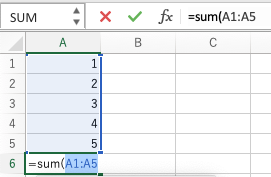
\includegraphics[width=10cm]{sum.png}
  \caption{総和を計算したいセルを選択した状態.}
  \label{fig:sum}
\end{figure}

同じやり方で,平均,分散,標準偏差が計算できます.平均なら``sum''の部分を``mean''.

\paragraph{演習}

csvの平均,分散を求めよ.
csvの平均,中央値を求めよ.そして,平均値と中央値の差について考察せよ.



\subsection{度数分布表とヒストグラム}

\paragraph{演習}
csvデータから度数分布表を書け.

\paragraph{演習}
度数分布表に基づきヒストグラムをかけ.



\section{考察}



\section{おまけ}

ファイル形式

確率分布

ガウス分布

不偏分散

\chapter{Excelによる統計処理2}

\section{目的}

エクセルにはデータを解析するための関数が多く用意されている.今回はその一部を用い,データ解析の初歩を学ぶ.

\section{原理}

\subsection{グラフ}

データの特徴を視覚的に把握するためにグラフを用います.
代表的なグラフの一つが前回取り扱ったヒストグラムです.
ヒストグラム以外にも様々なグラフが存在します.
今回は,折れ線グラフ,円グラフ,散布図を取り扱います.

\paragraph{折れ線グラフ}

値の時間変化の把握に用いられます.

\paragraph{円グラフ}

割合をは把握するために用いられます.
円グラフは合計で100\%にならなければなりません.

\paragraph{散布図}

データの値同士の関係性を知りたいときがあります.
値の関係性を見るために用いられます.
例えば,身長と体重の関係です.

\subsection{相関係数}

散布図では,視覚的に値同士の関係性を見ることができます.
しかし,定量的にどの程度関係しているか知りたいときには相関係数を使います.
相関係数は次の式で計算されます.

\subsection{散布図と回帰直線}



\section{実験}


\subsection{折れ線グラフ}



\paragraph{演習}
折れ線グラフ.



\subsection{散布図}

\paragraph{演習}
散布図をかけ.


\subsection{相関係数}

\paragraph{演習}
csvデータから相関係数を求めよ.

\subsection{共分散}

\paragraph{演習}
csvデータから相関係数を求めよ.

\subsection{演習}
散布図回帰直線

\paragraph{演習}

csvデータから散布図と回帰直線をかけ.


\section{考察}




\section{おまけ}
R,python

プロット
R,matplotlib,gnuplot


有料ならmatlabがある.

\section{レポートの出し方}

提出は電子データで送る.データ形式はpdfもしくはdocxとする.


\end{document}
